%\section{Ferramentas de Computação em Nuvem}
\section{Suporte Tecnológico}
Nesta Seção são apresentadas as ferramentas utilizadas para a consolidação da infraestrutura do LAPPIS. Basicamente, as ferramentas utilizadas englobam o nicho de computação em nuvem \textit{Cloudstack} e \textit{OpenNebula} e automatização da infraestrutura utilizando \textit{chef-solo} e \textit{chake}.
\subsection{Cloudstack}
\label{sub:subsecao}
Em um modelo simplificado, o \textit{Cloudstack} é composto de uma máquina de gerenciamento e dos recursos a serem gerenciados. Tais recursos compreende: faixa de endereços \textit{IP}, dispositivos \textit{storage}, servidores e \textit{VLAN'S}. Para implementação em uma configuração mínima, pode se utilizar uma máquina dedicada apenas para a interface de gerenciamento, mantendo o servidor físico apenas com o \textit{hypervisor}, ou utilizar o servidor físico executando a interface de gerenciamento e o \textit{hypervisor} simultaneamente como apresentado na Figura \ref{cloudstatck_minimal}. 

\begin{figure}[!htb]
\centering
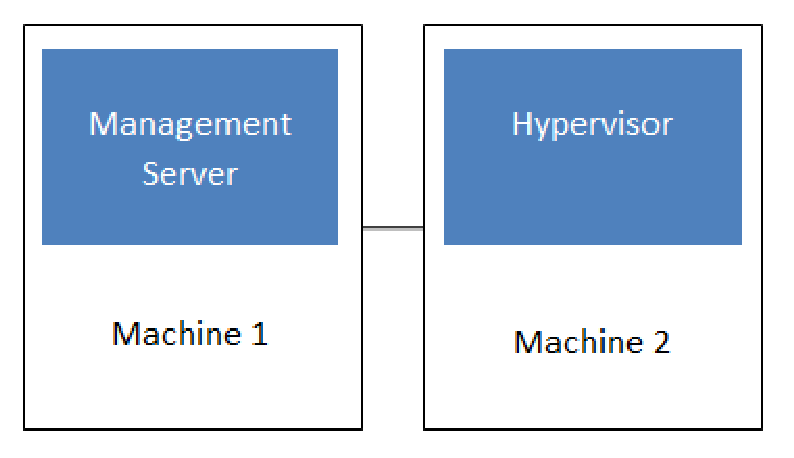
\includegraphics [keepaspectratio=true,scale=0.60]{figuras/cloudstack_minimal.eps}
\caption{Visão simplificada de uma instalação mínima do cloudstack}
\cite{cloudstack}.
\label{cloudstatck_minimal}
\end{figure}

Em modelo mais complexo, o \textit{Cloudstack} apresenta seu pontencial de disponibilidade escalabilidade e gerenciamento. Proporcionando uma modelagem de várias infraestruturas em nuvens em uma determinada região. Desse modo o \textit{Cloudstack} possui os seguintes níveis de abstrações \cite{shape}:

\begin{itemize}
\item \textbf{Regiões:} são a primeira e maior unidade de escala de uma implementação de uma \textit{cloud} com \textit{CloudStack}. Uma Região consiste em multiplas Zonas de Disponibilidade, a segunda maior unidade de escala.
\item \textbf{Zonas: } Tipicamente existe apenas uma Zona por \textit{Data Center} e cada Zona contem PODs, \textit{hosts} e \textit{storage.}
\item \textbf{Pods: } PODs tem propriedades lógicas e físicas com componentes como endereçamento IP e algoritmo de alocação de máquinas virtuais sendo influenciados por PODs dentro de uma Zona.
\item \textbf{Clusters: } São simples grupos de servidores homogêneos combinados com um Storage Primário. Cada Cluster utiliza um mesmo tipo de hypervisor mas em uma Zona pode coexistir combinações de todos os hypervisores suportados. Cada \textit{cluster} utiliza um mesmo tipo de \textit{hypervisor} mas em uma Zona pode coexistir combinações de todos os \textit{hypervisores} suportados.
\item \textbf{Hosts: } Responsável por disponibilizar a camada de computação real em que Máquinas Virtuais são executadas.
\item \textbf{Storage Primário: }  onde os discos das Máquinas Virtuais residem e pode ser utilizado o disco local de um \textit{host} ou um \textit{storage} compartilhado como \textit{NFS, iSCSI, Fiber Channel}, etc.
\item \textbf{Storage Secundário:} onde é armazenado os \textit{templates} de máquinas virtuais, arquivos ISO e \textit{snapshots} e é utilizado o protocolo NFS para este \textit{storage}.
\end{itemize}

A abstração desses níveis e como eles são alocados, são apresentados na Figura \ref{diagramacloudstack}.

\begin{figure}[!htb]
\centering
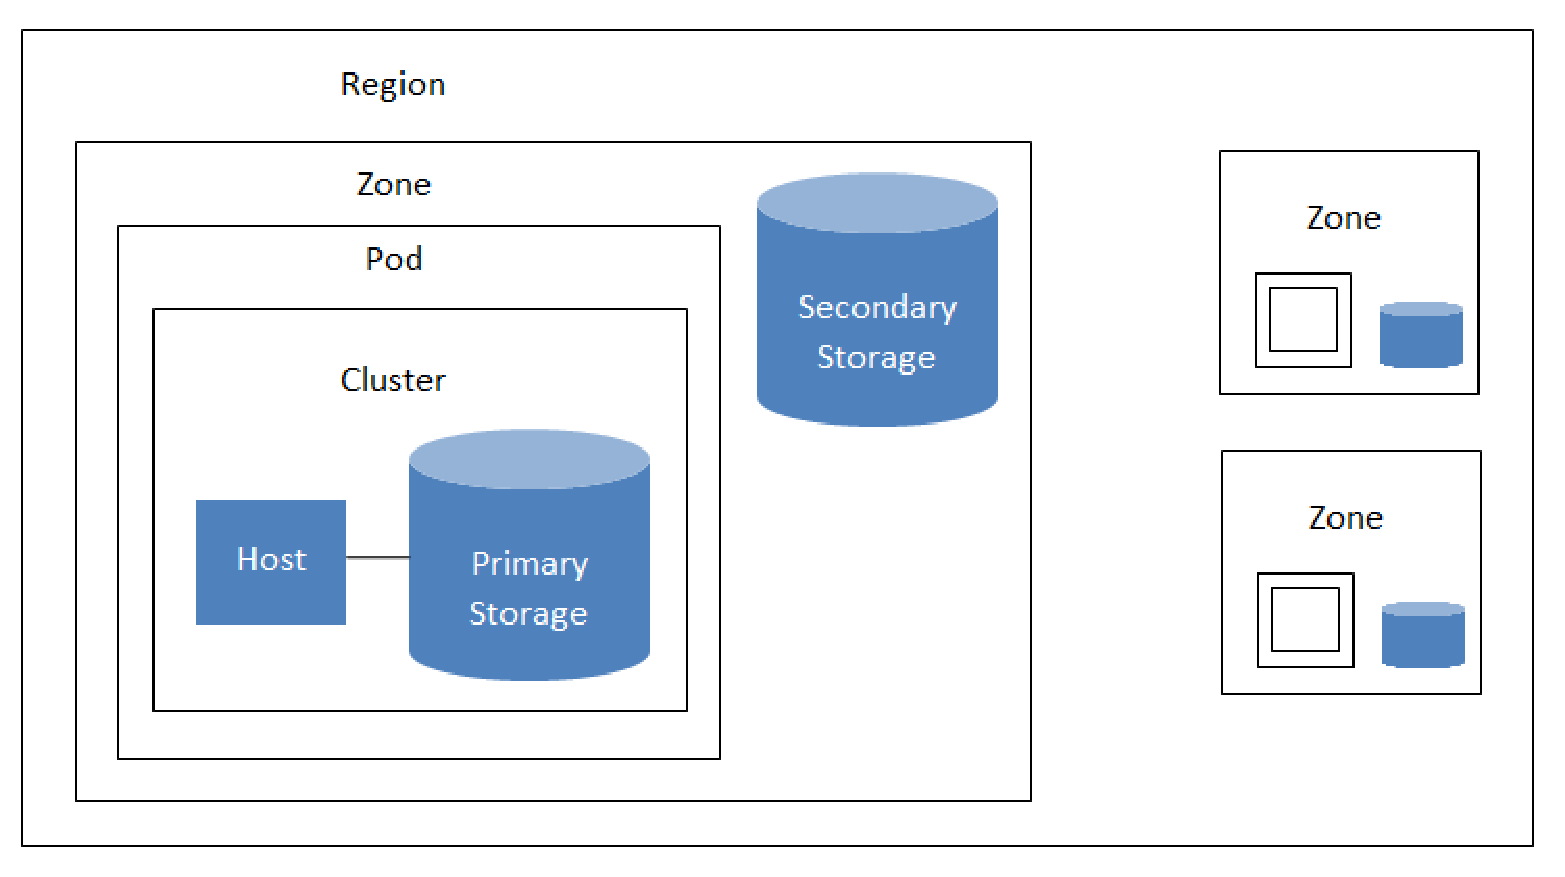
\includegraphics [keepaspectratio=true,scale=0.50]{figuras/cloudstack_structure.eps}
\caption{Visão geral da infraestrutura do \textit{Cloudstack}}
\cite{cloudstack}.
\label{diagramacloudstack}
\end{figure}

\subsection{OpenNebula}
O \textit{OpenNebula}, assim como o \textit{Cloudstack}, é uma ferramenta de código aberto que emergiu como um projeto de pesquisa em 2005 tendo seu primeiro lançamento público em março de 2008. Oferece uma solução simples mas repleta de funcionalidades para construir e gerenciar nuvens corporativas e \textit{data centers} virtuais. Além disso, combina tecnologias de virtualização existentes com funcionalides avançadas para fornecimento automático e elasticidade, seguindo uma abordagem \textit{bottom-up}, guiado pelas reais necessidades de adminstradores de sistemas e \textit{devops}\cite{opennebula}.

Em uma configuração mínima, a arquitetura do \textit{OpenNebula} é composta por três componentes: \textit{hosts}, \textit{datastores} e \textit{front-end}. Essa arquitetura é apresentada na Figura \ref{diagramaopennebula}. O \textit{front-end} é a máquina responsável por disponibilizar a interface de gerenciamento. Através da rede, monitora os \textit{hosts} e máquinas virtuais, bem como inicia operações relacionadas com máquinas virtuais e \textit{datastores}. O \textit{worker node} é  servidor físico propriamente dito, responsável pela criação de máquinas virtuais, é nesta máquina onde o \textit{hypervisor} será instalado. Por fim, o \textit{datastore} é o \textit{storage} utilizado como repositório de imagens e para manter os discos das máquinas virtuais em execução. Não precisa ser necessariamente um \textit{storage} dedicado, podendo ser uma máquina física com mais capacidade de disco ou até mesmo sendo um dos próprios \textit{hosts}.  

\begin{figure}[!htb]
\centering
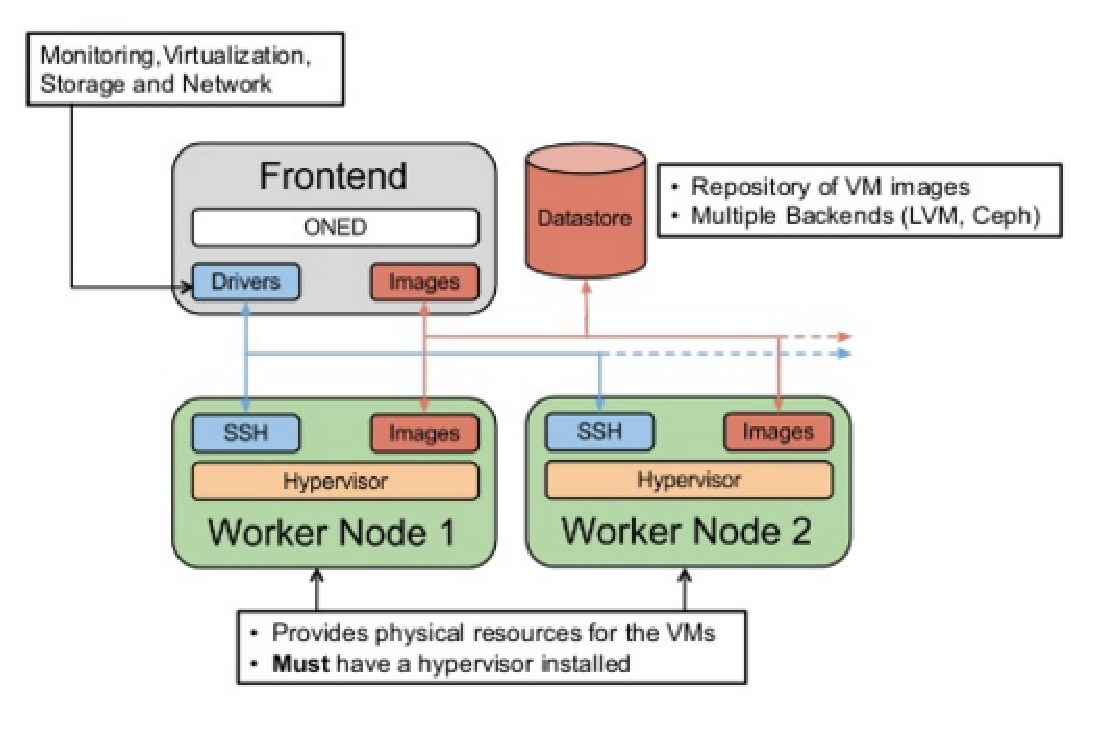
\includegraphics [keepaspectratio=true,scale=0.70]{figuras/opennebula_instalation.eps}
\caption{Visão geral da infraestrutura do OpenNebula}
\cite{opennebula}.
\label{diagramaopennebula}
\end{figure}

O \textit{System Datastore} é uma abstração do OpenNebula que é responsável por manter os discos das máquinas virtuais em execução. Possui três tipos\cite{opennebula}:

\begin{itemize}
\item \textit{\textbf{shared}} - O \textit{System Datastore} é compartilhado entre todos os outros hots usando \textit{NFS}, por exemplo.
\item \textit{\textbf{vmfs}} - Necessário quando o \textit{hypervisor} utilizado é o \textit{VMware}. Uma versão da opção \textit{shared} voltada para o sistemas de arquivos do \textit{VMware}.
\item \textit{\textbf{ssh}} - Nesse caso, cada host possui seu próprio \textit{System Datastore}.
\end{itemize}

As Figuras \ref{ssh_datastore} e \ref{shared_datastore}, apresentam uma abstração do \textit{System Datastore} quando configurados como \textit{shared} e \textit{ssh}, respectivamente. Nota-se, que na opção \textit{shared}, o \textit{System Datastore} é centralizado no próprio \textit{Datastore}, isso promove melhor desempenho na criação de máquinas virtuais. Entretanto, é necesário uma infraestrutura que possibilite uma boa velocidade de tráfego em rede, para que não haja perda de desempenho nas máquinas virtuais. Já na opção \textit{ssh}, o \textit{System Datastore} é mantido localmente não havendo riscos de perda de desempenho da máquina virtual por tráfego de rede, entretanto leva-se mais tempo para criação de máquinas virtuais do que na opção \textit{shared}, dado que, a imagem da máquina virtual será transferida do \textit{Datastore} para o servidor de destino.
\begin{figure}[!htb]
\centering
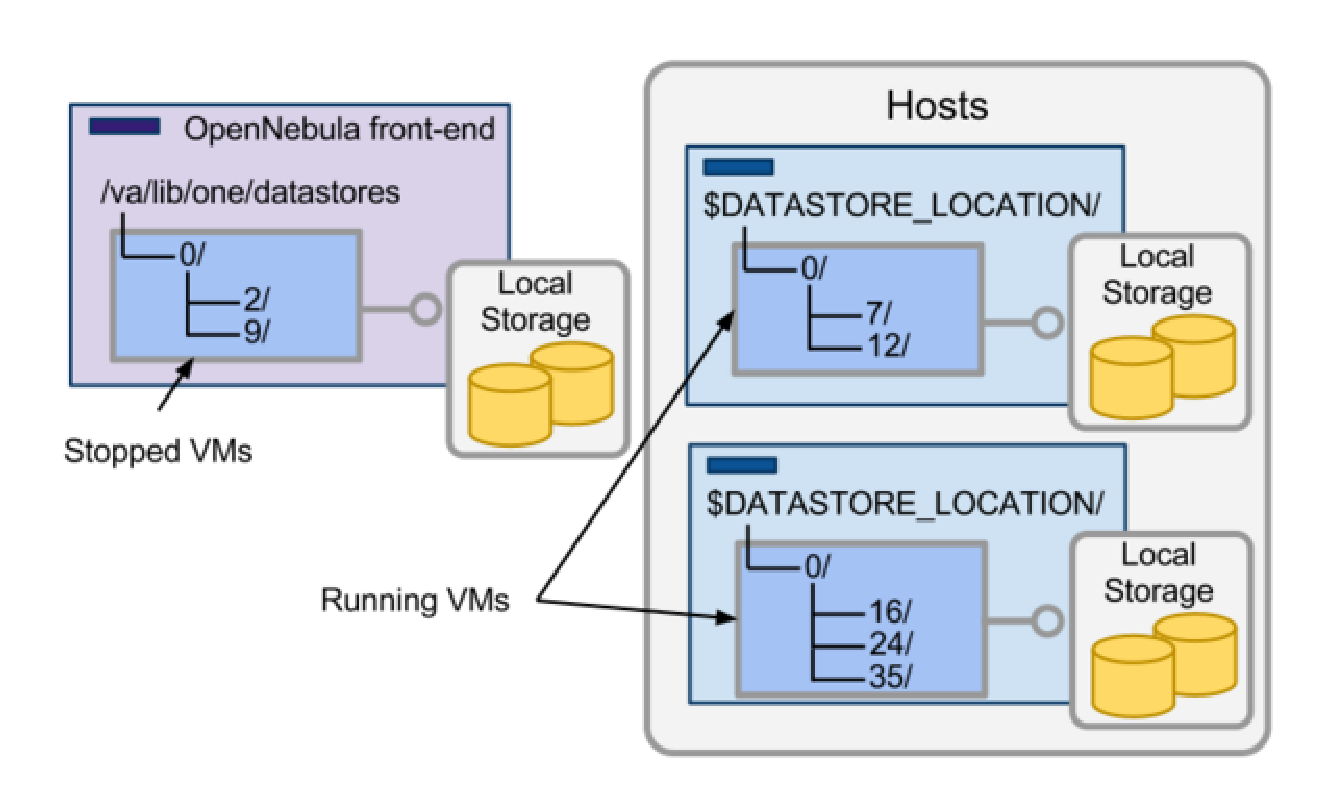
\includegraphics [keepaspectratio=true,scale=0.60]{figuras/ssh_datastore.eps}
\caption{Funcionamento do \textit{System Datastore} na configuração \textit{SSH}.}
\cite{opennebula}.
\label{ssh_datastore}
\end{figure}

\begin{figure}[!htb]
\centering
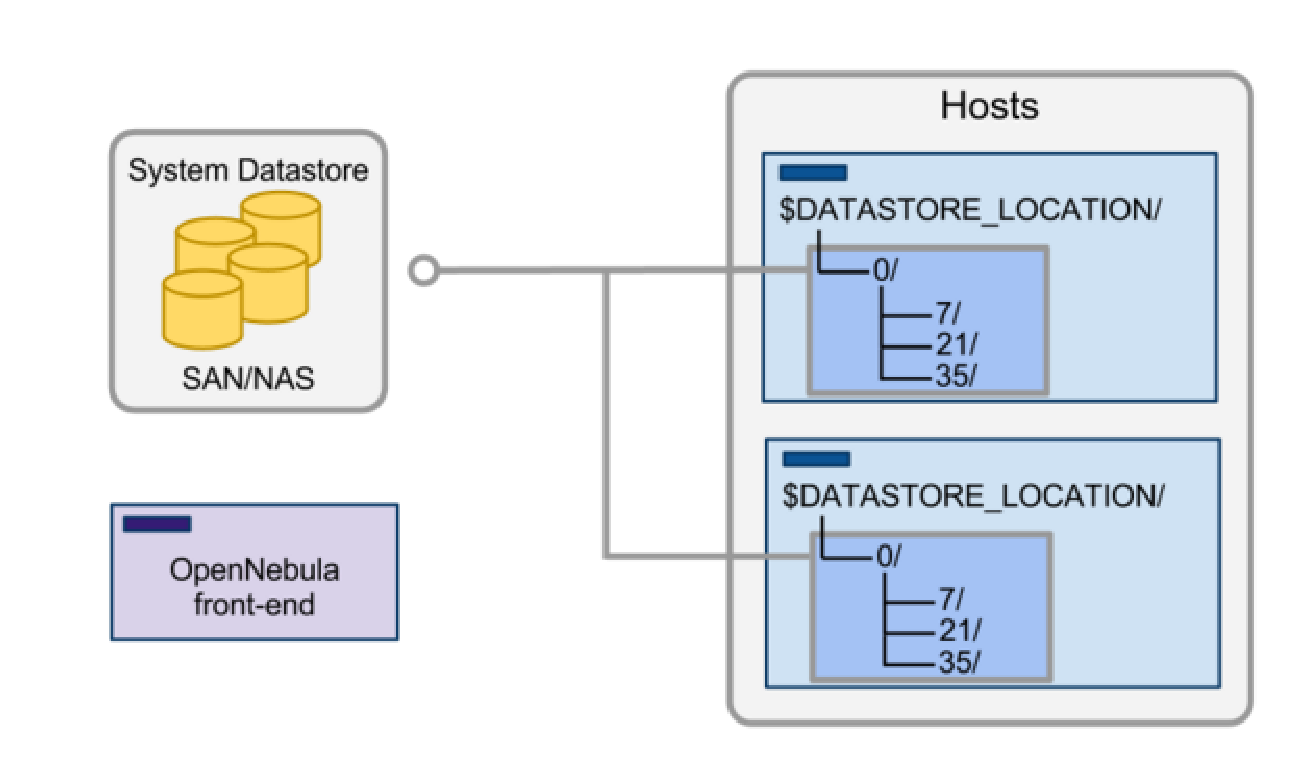
\includegraphics [keepaspectratio=true,scale=0.60]{figuras/shared_datastore.eps}
\caption{Funcionamento do \textit{System Datastore} na configuração \textit{shared}. }
\cite{opennebula}.
\label{shared_datastore}
\end{figure}

O \textit{OpenNebula} possui modelos de implementação tanto para nuvens privadas mais simplifcadas quanto para ambientes de infraestrutura mais complexos. Desse modo, para poucos servidores, a implementação do \textit{OpenNebula} é efetuada sem necessidade de ter que se preocupar elementos voltados para uma infraestrutura maior, que no caso do OpenNebula é chamada de Federação. Entretanto, para locais ou empresas que possuem múltiplos \textit{data centers}, que por sua vez, possuem vários \textit{clusters} de servidores, o \textit{OpenNebula} prover funcionalidades que colaboram para que vários data centers separados regionalmente possam ser gerenciados a partir de uma interface em nuvem com acesso externo. 

 A Figura \ref{opennebulafederation} apresenta uma abstração de Federação composta por vária instâncias do \textit{OpenNebula}. Cada instância do \textit{OpenNebula} é denominada de zona, desse modo em uma infraestrutura com múltiplas zonas pode ser configuradas como uma Federação. Assim, tem-se um compartilhamento da base de dados entre as zonas(Usuários, grupos). Nessa configuração, uma das zonas tem o papel de \textit{master}, ao qual é o responsável por escrever as informações na base dados, mantendo assim a consistência nos dados\cite{opennebula}.

\begin{figure}[!htb]
\centering
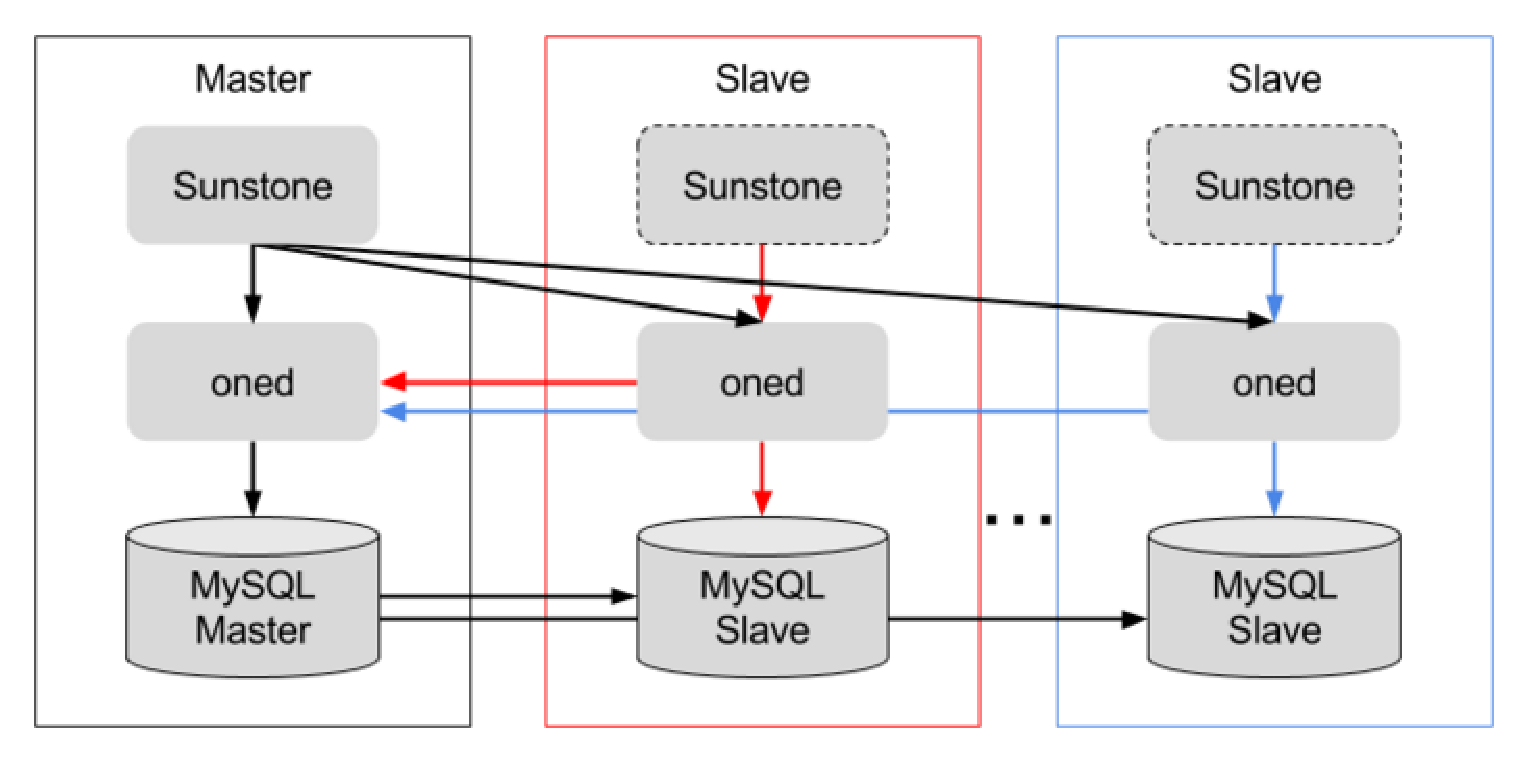
\includegraphics [keepaspectratio=true,scale=0.50]{figuras/opennebula_zone.eps}
\caption{Arquitetura de implantação por zonas}
\cite{opennebula}.
\label{opennebulafederation}
\end{figure}

\subsection{Comparativo entre as ferramentas de Plataforma em nuvem}

Nesta Seção é apresentado um breve comparativo entre as ferramentas \textit{OpenNebula} e \textit{Cloudstack} baseado no trabalho de \citeonline{salam}. O \textit{OpenNebula} tem como pontos fortes a flexibilidade e escalabilidade o que proporciona um certo dinanismo na adição de novos recursos. Já o \textit{Cloudstack} provê uma API que proporciona facilidades no que diz respeito a integração de outras ferramentas, possibilitando bons mecanismos para configuração da plataforma como um todo \cite{salam}. Entretanto, dos fatores apresentados na Tabela \ref{cloud_comparison}, a robustez contra erros foi decisivo para escolha em favor do OpenNebula, dado que, como é relatado no apêndice \ref{cap:estudo_caso}, o \textit{Cloudstack} mostrou-se bastante instável e intolerante a erros.

\begin{table}[!h]
\centering
\caption{Comparativo entre \textit{Cloudstack} e \textit{OpenNebula}}
\label{cloud_comparison}
\cite{salam}.
\resizebox{1.0\textwidth}{!}{
\begin{tabular}{|c|c|c|ll}
\cline{1-3}
\multicolumn{1}{|l|}{}                                                                     & OpenNebula                                                                                                                                     & Cloudstack                                                                                                                                    &  &  \\ \cline{1-3}
Arquitetura                                                                                & \begin{tabular}[c]{@{}c@{}}Árvore de módulos contendo\\  todos os componentes\end{tabular}                                                     & Servidor de Gerenciamento Central                                                                                                             &  &  \\ \cline{1-3}
Linguagem de Programação                                                                   & Java, Ruby                                                                                                                                     & Java, Python                                                                                                                                  &  &  \\ \cline{1-3}
Modelo de nuvem suportado                                                                  & Pública, Privada e Híbrida                                                                                                                     & Pública, Privada                                                                                                                              &  &  \\ \cline{1-3}
Hypervisor Suportado                                                                       & VMware, LXC, KVMand Xen                                                                                                                        & \begin{tabular}[c]{@{}c@{}}libvirt, hyper-V, VMware, \\ XenServer 6.2,\\ baremetal, docker,  Xen,\\   LXC via libvirt\end{tabular}            &  &  \\ \cline{1-3}
Transferência de dados                                                                     & NFS or Secure Copy(SCP)                                                                                                                        & \begin{tabular}[c]{@{}c@{}}Fornece uma ponte\\  entre os usuários finais\\  e a Área de armazenamento\end{tabular}                            &  &  \\ \cline{1-3}
Area de aplicação                                                                          & \begin{tabular}[c]{@{}c@{}}Grande companias comerciais \\ e instituições públicas\end{tabular}                                                 & \begin{tabular}[c]{@{}c@{}}Pequenas companias comerciais\\  e de pesquisa\end{tabular}                                                        &  &  \\ \cline{1-3}
Interface com o usuário                                                                    & Linha de comando \footnotemark[1]                                                                                                                              & \begin{tabular}[c]{@{}c@{}}Interface web baseada no AJAX, \\ gerencia requisições de sistemas\\  para administadores e usuários.\end{tabular} &  &  \\ \cline{1-3}
Licença                                                                                    & Apache2                                                                                                                                        & Apache2                                                                                                                                       &  &  \\ \cline{1-3}
Robustez contra erros                                                                      & \begin{tabular}[c]{@{}c@{}}Banco permanente para guardar\\  informaçõe sobre servidores, redes e VMs\end{tabular}                              & Limitado e centralizado                                                                                                                       &  &  \\ \cline{1-3}
Sistema operacional                                                                        & CentOS, Debian, OpenSUSE                                                                                                                       & \begin{tabular}[c]{@{}c@{}}CentOS,  Debian,  Fedora,  \\ RHEL, openSUSE, Ubuntu\end{tabular}                                                  &  &  \\ \cline{1-3}
Segurança                                                                                  & \begin{tabular}[c]{@{}c@{}}O frontend gera uma chave codificada\\  pública/privada emparelhada\\  para autenticação com o usuário\end{tabular} & \begin{tabular}[c]{@{}c@{}}Integrado com LDAP e Active Directory,\\  inclui diversos niveis de acesso\end{tabular}                            &  &  \\ \cline{1-3}
\begin{tabular}[c]{@{}c@{}}Compatibilidade com serviços\\  em nuvem da Amazon\end{tabular} & EC2, S3                                                                                                                                        & EC2, S3                                                                                                                                       &  &  \\ \cline{1-3}
\end{tabular}}
\end{table}

\footnotetext[1]{\textit{OpenNebula} também prover uma interface \textit{web}, possui um módulo responsável por isso chamado \textit{Sunstone}}

\subsection{Automatização da Infraestrutura}
O \textit{Chef} é um \textit{Framework} que tem como objetivo transformar uma complexa infraestrutura em código, tornando mais fácil a disponiblização de aplicações em qualquer ambiente seja ele físico ou virtual \cite{chef}. É composto pelo \textit{Chef Client} e pelo \textit{Chef Server}, sendo que o \textit{Chef Client} é responsável por efetuar as configurações necessárias na máquina pretendida a partir de informações localizadas e gerenciadas pelo \textit{Chef Server}. As configurações são feitas a partir de arquivos denominados de recursos e receitas \textit{Chef}. Os recursos descrevem algum pedaço da infraestrutura tal como um arquivo, template ou pacote. A receita \textit{Chef} é um arquivo que contém os recursos relacionados à configuração de um servidor \textit{web} ou de banco de dados. No código \ref{codigoChef}, é apresentado um exemplo de uma receita \textit{Chef}. Na linha 1 é feita a instalação de um servidor \textit{apache} usando a diretiva \textit{package} que se equivale a um \textit{yum install} ou \textit{apt-get install}. Nas linha 3 a 5 usa-se o recurso \textit{service} para habilitar e iniciar o serviço do \textit{apache}. Por fim, o recurso \textit{template} define um arquivo de configuração, no caso \textit{index.html.erb}, já pronto a ser utilizado na máquina alvo no endereço \textit{/var/www.html.index.html}. Um meio de se utilizar o \textit{Chef client} sem ter que o usar o \textit{Chef Server} é usar a versão código aberto do \textit{Chef client}, o \textit{Chef Solo}.

O \textit{Chake} é uma ferramenta que ajuda a gerenciar múltiplos ambientes sem a necessidade de se utilizar o \textit{Chef Server}. As configurações são geralmente implantadas via \textit{rsync} com o auxílio do \textit{SSH}, e aplicadas invocando o \textit{Chef Solo} em cada ambiente. O uso dessas ferramentas contribui para gerencia do serviços oferecidos, promovendo também um meio de compartilhamento de conhecimento através do código.

Dentre outras ferramentas de automatização o \textit{Chef} foi a solução que demonstrou maior maturidade e robustez, o uso do \textit{Chake} possibilita o uso da versão livre do \textit{Chef Client}, o \textit{Chef Solo}.

\begin{lstlisting}[caption={Código exemplo de uma receita Chef}, label=codigoChef]
package 'httpd'

service 'httpd' do
 action [:enable, :start]
end

template '/var/www/html/index.html' do
  source 'index.html.erb'
end
\end{lstlisting}

A escolha do \textit{Chef} deve se ao fato de ser uma ferramenta bastante consolidada no que diz respeito a automatização da infraestrutura.  O uso de uma linguagem de domínio específico para especificação de recursos utilizando o \textit{ruby} como linguagem de referênncia, facilita na documentação através do código.
